\documentclass[10pt,a4paper]{article}
\usepackage[margin=1.8cm,top=1.6cm,bottom=1.7cm]{geometry}
\usepackage{times}
\usepackage[T1]{fontenc}
\usepackage{microtype}
\usepackage{amsmath,amssymb}
\usepackage{graphicx}
\usepackage{booktabs}
\usepackage[numbers,sort&compress]{natbib}
\usepackage{xcolor}
\usepackage[hidelinks]{hyperref}
\usepackage{xurl} % lets long URLs in the checklist break across lines
\usepackage{titlesec}
\usepackage{enumitem}
\usepackage{caption}
\captionsetup{font=small,labelfont=bf,skip=3pt}
\titleformat{\section}{\normalsize\bfseries}{\thesection}{0.6em}{}
\titlespacing*{\section}{0pt}{5pt}{2pt}
\setlength{\parskip}{0pt}
\setlength{\bibsep}{1pt}
\setlist{nosep,leftmargin=1.2em}

\title{\vspace{-0.6cm}\large\bfseries Retrieval Survives, Choice Collapses:\\
Induction Heads under Recursive Synthetic Training}
\author{\normalsize Sibonelo Mlambo (536187)\\
\small School of Computer Science and Applied Mathematics, University of the Witwatersrand\\
\small COMS4054A/COMS7062A/COMS7066A Natural Language Processing, Project 1}
\date{\vspace{-0.9cm}}

\begin{document}
\maketitle

\begin{abstract}
\noindent We train two-layer Transformers on the in-context symbol--value task of Singh et al.\ and retrain each generation on labels sampled from its predecessor. A pilot with a short training budget never left the pre-induction plateau, so we first make induction heads form at generation~0 (100\% accuracy, causal head-ablation drops up to 70 points). Predicting one value shows no collapse. When the model must also choose a next symbol and give its value, consistency falls linearly (99.4\%$\to$94.8\% over five generations) as probability leaks to symbols absent from the context (0.7\%$\to$4.9\%). Retrieval is untouched: values of shown symbols stay $\geq$99.6\% correct and induction attention stays at ceiling. Direct logit attribution traces the leak to a shrinking preference for in-context symbols at the choice step, 78\% of it in the layer-2 heads. Keeping half of every generation's labels real stops the drift at a ceiling predicted by a simple error-propagation model.
\end{abstract}

\section{Introduction}
In-context learning (ICL) lets a Transformer infer a mapping from its prompt without weight updates, and induction heads are a well-understood mechanism for it \citep{olsson2022,singh2024}. Model collapse is the degradation of models trained on earlier models' outputs \citep{shumailov2023,shumailov2024}. We ask whether recursive training damages the ICL \emph{mechanism} or only what the model chooses to produce. On a task with a known circuit we show that (i) a short training budget yields a non-induction heuristic that must be ruled out first; (ii) a fully context-determined target does not collapse; (iii) when the target includes a free choice, collapse appears as a steadily weakening preference for in-context symbols, located mostly in layer-2 heads, while retrieval stays intact; and (iv) mixing in real data bounds the damage, as a simple error-propagation model predicts.

\section{Background}
In a two-layer induction circuit a layer-1 \emph{previous-token head} copies each token's predecessor into its residual stream, and a layer-2 \emph{induction head} matches the current token against those keys and copies the token that followed \citep{olsson2022}. On this symbol--value task the circuit forms in an abrupt phase transition after a long loss plateau \citep{singh2024}. Recursive training compounds sampling and approximation error, so learned distributions lose their tails and drift \citep{shumailov2023,shumailov2024}. Circuit claims should rest on causal interventions, not attention maps alone \citep{conmy2023}, and interpretable units can be traced back to the training data that formed them \citep{chen2026}. Under recursion that data is itself model output.

\section{Method}
\textbf{Task.} Each sequence draws a fresh bijection between 8 symbol and 8 value tokens. The context is \texttt{BOS}, six symbol--value pairs (symbols with replacement) and a query symbol shown earlier. The \emph{base} target is the query's value. The \emph{extended} target adds a next symbol, drawn uniformly from the distinct shown symbols, and its value. Our pilot drew it from all 8 symbols, making its value unknowable in 45\% of cases. The redesign keeps every target inferable and gives the symbol choice a known uniform reference.

\textbf{Model and training.} A 2-layer causal Transformer (4 heads, width 64, MLP 128, pre-LayerNorm, learned positions, tied embeddings) is trained with AdamW (weight decay $10^{-4}$, batch 128) on cross-entropy over target tokens. We use 50k/2k/2k train/validation/test sequences and keep the checkpoint with the lowest validation loss (max.\ 20 epochs, patience 6). Learning rate $\in\{3{\cdot}10^{-4},10^{-3},3{\cdot}10^{-3}\}$ and training size $\in\{3\text{k},50\text{k}\}$ are selected on validation data only.

\textbf{Recursion.} Generation~0 trains on real labels. Generation $g{\geq}1$ is a freshly initialised model trained on the same contexts, where a fraction $f$ of labels is sampled at $T{=}1$ from generation $g{-}1$ and the rest stay real. We run $f{=}1$ for both tasks and $f{=}0.5$ for the extended task, each for 6 generations $\times$ 3 seeds. Validation and test labels are always real.

\textbf{Metrics.} \emph{Pair consistency} is the fraction of sampled extended outputs whose symbol is shown and whose value matches it. Exact match is capped near 0.24 because the next symbol is random by design. The \emph{induction score} is the attention from the query to values following earlier occurrences of the query symbol (uniform attention over values scores 0.27). Head \emph{ablation} zeroes one head and records the drop in first-value accuracy. \emph{Leaked mass} is the probability placed on unshown symbols at the choice step. For \emph{direct logit attribution} (DLA) we freeze the final LayerNorm scale and split the choice-step logits exactly into contributions from embeddings, each head and each MLP. For each component we report the mean logit it gives shown minus unshown symbols.

\begin{figure}[t]
\centering
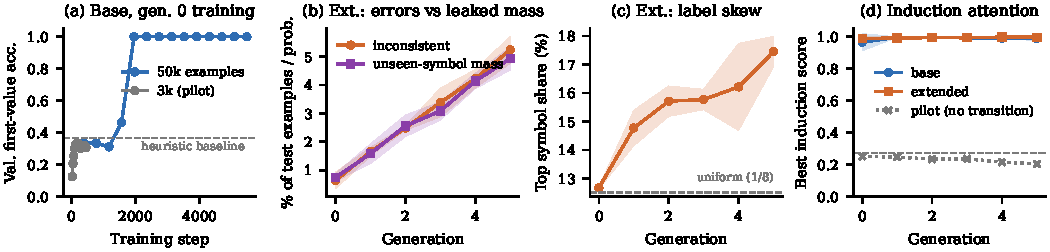
\includegraphics[width=\linewidth]{figures/main_figure.pdf}
\caption{(a) Generation-0 validation accuracy: with 3k examples training stops on the plateau, while with 50k the induction transition occurs at $\approx$1{,}600--2{,}000 steps. (b) Extended task, $f{=}1$: inconsistent pairs and mass on unshown symbols grow together; with 50\% real labels (green) errors level off. (c) DLA at the choice step ($f{=}1$): the shown$-$unshown logit gap shrinks, mostly in layer-2 heads. (d) Induction attention stays at ceiling; the pilot stayed at the uniform baseline (dashed). Bands: $\pm$1 SD over 3 seeds.}
\label{fig:main}
\end{figure}

\section{Results}
\textbf{Pilot and tuning.} With 3k examples ($\approx$600 steps) generation-0 accuracy was $32.0\pm3.1\%$, between the heuristics ``copy a random context value'' (25.8\%) and ``copy the most frequent value'' (36.8\%), with induction scores (0.24) at the uniform baseline. Every learning rate stayed at 30--34\% with 3k examples. With 50k, $10^{-3}$ and $3{\cdot}10^{-4}$ reached 100\% and $3{\cdot}10^{-3}$ stalled at 70\%. We chose $10^{-3}$, which crossed 99\% fastest (1{,}955 steps; Fig.~\ref{fig:main}a).

\textbf{Base task: no collapse.} All 18 base models score 100\% at every generation, their synthetic labels are $\geq$99.998\% correct, and induction scores stay at 0.90--1.00.

\textbf{Extended task: choice collapses, retrieval does not.} First-value accuracy stays at 100\%, but pair consistency falls by 0.9 points per generation (Fig.~\ref{fig:main}b, Table~\ref{tab:res}). Nearly every failure is an unshown symbol. When the symbol is shown its value is correct in $\geq$99.6\% of cases, and greedy decoding stays 100\% consistent. Leaked mass tracks the errors (0.7\%$\to$4.9\%), and the training labels skew: the top symbol's share rises from 12.7\% to 17.5\%. Clean-test loss shows the same drift more faintly: perplexity rises from 1.645 to 1.699 ($f{=}0.5$: 1.658), against a floor above 1 set by the random next symbol, while base-task perplexity stays at 1.000.

\textbf{Mechanism.} Induction scores (0.97--1.00) and causal ablations (largest single-head drop 9--70 points in every model) show an intact retrieval circuit. DLA shows what changes instead: the total logit gap favouring shown symbols shrinks from $5.26\pm0.19$ to $3.04\pm0.11$, monotonically in every seed. The layer-2 heads account for 78\% of this ($3.22\to1.49$), layer-1 heads change less and less consistently ($1.98\to1.60$), and MLPs and embeddings contribute almost nothing (Fig.~\ref{fig:main}c). Token embeddings give a shown$-$unshown gap below 0.01 logits in every generation, and the spread of their per-symbol bias does not grow (SD 0.12--0.24), so the leak is not stored in how symbols are embedded. No component's symbol-specific bias grows, so the skew reflects leaked mass flowing to pre-existing preferences rather than a new symbol prior.

\textbf{Mixing real data.} With $f{=}0.5$, consistency settles at 98.1--98.5\% from generation~2 onwards, leaked mass at 1.7--1.8\% and the logit gap at 4.2--4.3. Generation~0 is identical in both runs, confirming the comparison is controlled.

\begin{table}[t]
\centering\small
\caption{Clean-test results (mean $\pm$ SD over 3 seeds). Extended rows use $f{=}1$ unless marked.}
\label{tab:res}
\begin{tabular}{llccc}
\toprule
Task & Metric & Gen.~0 & Gen.~5 ($f{=}1$) & Gen.~5 ($f{=}0.5$) \\
\midrule
Base & First-value accuracy & $1.000\pm0.000$ & $1.000\pm0.000$ & -- \\
Extended & First-value accuracy & $1.000\pm0.000$ & $1.000\pm0.000$ & $1.000\pm0.000$ \\
Extended & Sampled pair consistency & $0.994\pm0.003$ & $0.948\pm0.005$ & $0.985\pm0.004$ \\
Extended & Leaked mass on unshown symbols & $0.007\pm0.001$ & $0.049\pm0.004$ & $0.017\pm0.002$ \\
Extended & Unshown symbols in training labels & $0.000\pm0.000$ & $0.041\pm0.002$ & $0.009\pm0.001$ \\
Extended & Shown$-$unshown logit gap (DLA) & $5.26\pm0.19$ & $3.04\pm0.11$ & $4.26\pm0.16$ \\
Extended & Best induction score & $0.988\pm0.015$ & $0.997\pm0.002$ & $0.994\pm0.006$ \\
\bottomrule
\end{tabular}
\end{table}

\section{Discussion and limitations}
A context-determined lookup is a fixed point of recursion: a perfect model emits perfect labels. A uniform choice is not. Each model puts a little mass, $\delta$, on unshown symbols, sampling turns it into labels, and the next model learns those labels as legitimate data. This coincides with a shrinking shown-symbol preference in the layer-2 heads, and the unshown-label rate follows $L_{g+1}=f(L_g+\delta)$. With $\delta\approx0.76\%$ (the generation-1 label rate at $f{=}1$), this predicts linear growth $L_5=5\delta\approx3.8\%$ for $f{=}1$ (observed 4.1\%) and a ceiling $f\delta/(1-f)=\delta\approx0.76\%$ for $f{=}0.5$ (observed 0.9\%). Unlike the tail loss of \citep{shumailov2024}, the damage here is \emph{spurious} tail mass that grows while the mode, greedy decoding and the induction circuit stay perfect. The circuit does not break. What erodes is how strongly the layer-2 heads restrict the free choice to context symbols, and real data caps that erosion. Collapse in ICL can therefore hide behind intact circuits and perfect accuracy, and only distributional metrics on sampled outputs expose it.

\textbf{Limitations.} Only labels are recursive (contexts stay real), at $T{=}1$. Five generations, three seeds, one mixing level, 8 symbols and 2 layers limit generality. Early stopping on real validation data gives each generation some real signal. DLA freezes the LayerNorm scale and attributes logits, not the attention weights behind them. Ablation of single heads understates redundancy. Future work: path patching to see which attention edges carry the weakened preference, and more values of $f$ and $T$.

\clearpage
\begin{thebibliography}{9}\small
\bibitem{chen2026} J.~Chen, Y.~Luo, and L.~Pan. Mechanistic data attribution: Tracing the training origins of interpretable LLM units. \emph{arXiv preprint arXiv:2601.21996}, 2026.
\bibitem{conmy2023} A.~Conmy, A.~Mavor-Parker, A.~Lynch, S.~Heimersheim, and A.~Garriga-Alonso. Towards automated circuit discovery for mechanistic interpretability. \emph{Advances in Neural Information Processing Systems}, 36:16318--16352, 2023.
\bibitem{olsson2022} C.~Olsson, N.~Elhage, N.~Nanda, N.~Joseph, N.~DasSarma, T.~Henighan, B.~Mann, A.~Askell, Y.~Bai, A.~Chen, et~al. In-context learning and induction heads. \emph{arXiv preprint arXiv:2209.11895}, 2022.
\bibitem{shumailov2023} I.~Shumailov, Z.~Shumaylov, Y.~Zhao, Y.~Gal, N.~Papernot, and R.~Anderson. The curse of recursion: Training on generated data makes models forget. \emph{arXiv preprint arXiv:2305.17493}, 2023.
\bibitem{shumailov2024} I.~Shumailov, Z.~Shumaylov, Y.~Zhao, N.~Papernot, R.~Anderson, and Y.~Gal. AI models collapse when trained on recursively generated data. \emph{Nature}, 631(8022):755--759, 2024.
\bibitem{singh2024} A.~K.~Singh, T.~Moskovitz, F.~Hill, S.~C.~Y.~Chan, and A.~M.~Saxe. What needs to go right for an induction head? A mechanistic study of in-context learning circuits and their formation. In \emph{International Conference on Machine Learning}, pp.~45637--45662. PMLR, 2024.
\end{thebibliography}

\section*{Contribution statement}
This is an individual submission. Sibonelo Mlambo (536187) carried out the experimental design, implementation, experiments, analysis, figures and writing.

\section*{Code and reproducibility}
Code, configurations, raw results and checkpoints accompany the submission. \texttt{tune.py} reproduces the hyper-parameter selection, \texttt{run\_study.py} the main study, \texttt{analyse\_leakage.py} and \texttt{analyse\_mechanism.py} the leaked-mass and attribution analyses, \texttt{configs/mix50.yaml} the mixing run, and \texttt{make\_figures.py} Figure~\ref{fig:main}. All experiments ran on CPU without a GPU. The main study (3 seeds $\times$ 2 tasks $\times$ 6 generations, 36 training runs on 50k sequences) takes about 2--2.5 hours on a 2-core CPU. The other reported experiments add 18 runs for the mixing ablation (extended task only), 6 runs for the tuning grid (three of them on 3k sequences) and 36 runs for the pilot on 3k sequences.

\section*{Broader impact}
Recursive training on generated data is a growing concern as model outputs enter training corpora. Our results suggest a practical lesson: collapse can grow while accuracy, greedy outputs and the underlying circuit all look intact, so monitoring should include distributional metrics on sampled outputs, and retaining real data limits the damage. The models are tiny and trained on synthetic tokens, so we see no direct path to misuse; the main risk is over-generalising these small-scale findings to production language models, which the limitations above caution against.

% ---- NeurIPS 2024 checklist: save the official file from Moodle as report/checklist.tex ----
\clearpage
\IfFileExists{checklist.tex}{% NeurIPS 2024 paper checklist (official questions and guidelines from neurips_2024.tex),
% answered for this extended abstract. Included by main.tex after the references.
% Answer macros as defined in neurips_2024.sty (main.tex does not load that style file).
\providecommand{\answerYes}[1][]{\textcolor{blue}{[Yes] #1}}
\providecommand{\answerNo}[1][]{\textcolor{orange}{[No] #1}}
\providecommand{\answerNA}[1][]{\textcolor{gray}{[NA] #1}}
\providecommand{\answerTODO}[1][]{\textcolor{red}{\bf [TODO]}}
\providecommand{\justificationTODO}[1][]{\textcolor{red}{\bf [TODO]}}

\section*{NeurIPS Paper Checklist}

\begin{enumerate}

\item {\bf Claims}
    \item[] Question: Do the main claims made in the abstract and introduction accurately reflect the paper's contributions and scope?
    \item[] Answer: \answerYes{}
    \item[] Justification: Every quantitative claim in the abstract and introduction is reported in Section~4 (Results), Figure~1 and Table~1, and was computed from the saved result files. The scope (a two-layer model, a synthetic symbol--value task, recursion over labels only) is stated in Section~3 (Method) and Section~5 (Discussion and limitations).
    \item[] Guidelines:
    \begin{itemize}
        \item The answer NA means that the abstract and introduction do not include the claims made in the paper.
        \item The abstract and/or introduction should clearly state the claims made, including the contributions made in the paper and important assumptions and limitations. A No or NA answer to this question will not be perceived well by the reviewers.
        \item The claims made should match theoretical and experimental results, and reflect how much the results can be expected to generalize to other settings.
        \item It is fine to include aspirational goals as motivation as long as it is clear that these goals are not attained by the paper.
    \end{itemize}

\item {\bf Limitations}
    \item[] Question: Does the paper discuss the limitations of the work performed by the authors?
    \item[] Answer: \answerYes{}
    \item[] Justification: Section~5 has a Limitations paragraph: only labels are recursive (contexts stay real), sampling is at $T{=}1$, and there are five generations, three seeds, one mixing level, 8 symbols and 2 layers. It also notes that early stopping on real validation data gives each generation some real signal, that DLA freezes the LayerNorm scale and attributes logits rather than attention weights, and that single-head ablation understates redundancy.
    \item[] Guidelines:
    \begin{itemize}
        \item The answer NA means that the paper has no limitation while the answer No means that the paper has limitations, but those are not discussed in the paper.
        \item The authors are encouraged to create a separate "Limitations" section in their paper.
        \item The paper should point out any strong assumptions and how robust the results are to violations of these assumptions (e.g., independence assumptions, noiseless settings, model well-specification, asymptotic approximations only holding locally). The authors should reflect on how these assumptions might be violated in practice and what the implications would be.
        \item The authors should reflect on the scope of the claims made, e.g., if the approach was only tested on a few datasets or with a few runs. In general, empirical results often depend on implicit assumptions, which should be articulated.
        \item The authors should reflect on the factors that influence the performance of the approach. For example, a facial recognition algorithm may perform poorly when image resolution is low or images are taken in low lighting. Or a speech-to-text system might not be used reliably to provide closed captions for online lectures because it fails to handle technical jargon.
        \item The authors should discuss the computational efficiency of the proposed algorithms and how they scale with dataset size.
        \item If applicable, the authors should discuss possible limitations of their approach to address problems of privacy and fairness.
        \item While the authors might fear that complete honesty about limitations might be used by reviewers as grounds for rejection, a worse outcome might be that reviewers discover limitations that aren't acknowledged in the paper. The authors should use their best judgment and recognize that individual actions in favor of transparency play an important role in developing norms that preserve the integrity of the community. Reviewers will be specifically instructed to not penalize honesty concerning limitations.
    \end{itemize}

\item {\bf Theory Assumptions and Proofs}
    \item[] Question: For each theoretical result, does the paper provide the full set of assumptions and a complete (and correct) proof?
    \item[] Answer: \answerNA{}
    \item[] Justification: The paper has no theorems. The error-propagation model $L_{g+1}=f(L_g+\delta)$ in Section~5 is a simple heuristic: its assumption (a constant per-generation leak $\delta$) is stated there, and its predictions are compared with the observed values rather than proved.
    \item[] Guidelines:
    \begin{itemize}
        \item The answer NA means that the paper does not include theoretical results.
        \item All the theorems, formulas, and proofs in the paper should be numbered and cross-referenced.
        \item All assumptions should be clearly stated or referenced in the statement of any theorems.
        \item The proofs can either appear in the main paper or the supplemental material, but if they appear in the supplemental material, the authors are encouraged to provide a short proof sketch to provide intuition.
        \item Inversely, any informal proof provided in the core of the paper should be complemented by formal proofs provided in appendix or supplemental material.
        \item Theorems and Lemmas that the proof relies upon should be properly referenced.
    \end{itemize}

    \item {\bf Experimental Result Reproducibility}
    \item[] Question: Does the paper fully disclose all the information needed to reproduce the main experimental results of the paper to the extent that it affects the main claims and/or conclusions of the paper (regardless of whether the code and data are provided or not)?
    \item[] Answer: \answerYes{}
    \item[] Justification: Section~3 specifies the task and data generation, the architecture, the optimiser and its settings, the data splits, early stopping, the hyper-parameter search, the recursion procedure (synthetic fraction $f$, temperature $T$, number of generations and seeds) and every metric. The exact configurations and random seeds are in the submitted \texttt{configs/} files.
    \item[] Guidelines:
    \begin{itemize}
        \item The answer NA means that the paper does not include experiments.
        \item If the paper includes experiments, a No answer to this question will not be perceived well by the reviewers: Making the paper reproducible is important, regardless of whether the code and data are provided or not.
        \item If the contribution is a dataset and/or model, the authors should describe the steps taken to make their results reproducible or verifiable.
        \item Depending on the contribution, reproducibility can be accomplished in various ways. For example, if the contribution is a novel architecture, describing the architecture fully might suffice, or if the contribution is a specific model and empirical evaluation, it may be necessary to either make it possible for others to replicate the model with the same dataset, or provide access to the model. In general. releasing code and data is often one good way to accomplish this, but reproducibility can also be provided via detailed instructions for how to replicate the results, access to a hosted model (e.g., in the case of a large language model), releasing of a model checkpoint, or other means that are appropriate to the research performed.
        \item While NeurIPS does not require releasing code, the conference does require all submissions to provide some reasonable avenue for reproducibility, which may depend on the nature of the contribution. For example
        \begin{enumerate}
            \item If the contribution is primarily a new algorithm, the paper should make it clear how to reproduce that algorithm.
            \item If the contribution is primarily a new model architecture, the paper should describe the architecture clearly and fully.
            \item If the contribution is a new model (e.g., a large language model), then there should either be a way to access this model for reproducing the results or a way to reproduce the model (e.g., with an open-source dataset or instructions for how to construct the dataset).
            \item We recognize that reproducibility may be tricky in some cases, in which case authors are welcome to describe the particular way they provide for reproducibility. In the case of closed-source models, it may be that access to the model is limited in some way (e.g., to registered users), but it should be possible for other researchers to have some path to reproducing or verifying the results.
        \end{enumerate}
    \end{itemize}


\item {\bf Open access to data and code}
    \item[] Question: Does the paper provide open access to the data and code, with sufficient instructions to faithfully reproduce the main experimental results, as described in supplemental material?
    \item[] Answer: \answerYes{}
    \item[] Justification: The full code is submitted with the paper, with \texttt{requirements.txt} and a \texttt{README.txt} that gives the exact command for tuning, the main study, the mixing ablation, each analysis and the figure. The data is synthetic and is regenerated from fixed seeds by the code, so no download is needed. Raw per-seed results and model checkpoints are also included.
    \item[] Guidelines:
    \begin{itemize}
        \item The answer NA means that paper does not include experiments requiring code.
        \item Please see the NeurIPS code and data submission guidelines (\url{https://nips.cc/public/guides/CodeSubmissionPolicy}) for more details.
        \item While we encourage the release of code and data, we understand that this might not be possible, so “No” is an acceptable answer. Papers cannot be rejected simply for not including code, unless this is central to the contribution (e.g., for a new open-source benchmark).
        \item The instructions should contain the exact command and environment needed to run to reproduce the results. See the NeurIPS code and data submission guidelines (\url{https://nips.cc/public/guides/CodeSubmissionPolicy}) for more details.
        \item The authors should provide instructions on data access and preparation, including how to access the raw data, preprocessed data, intermediate data, and generated data, etc.
        \item The authors should provide scripts to reproduce all experimental results for the new proposed method and baselines. If only a subset of experiments are reproducible, they should state which ones are omitted from the script and why.
        \item At submission time, to preserve anonymity, the authors should release anonymized versions (if applicable).
        \item Providing as much information as possible in supplemental material (appended to the paper) is recommended, but including URLs to data and code is permitted.
    \end{itemize}


\item {\bf Experimental Setting/Details}
    \item[] Question: Does the paper specify all the training and test details (e.g., data splits, hyperparameters, how they were chosen, type of optimizer, etc.) necessary to understand the results?
    \item[] Answer: \answerYes{}
    \item[] Justification: Section~3 gives the 50k/2k/2k train/validation/test split, AdamW with weight decay $10^{-4}$, batch size 128, at most 20 epochs with patience 6, and the learning-rate and training-size grid, which was selected on validation data only; the selection is reported in Section~4. Validation and test labels are always real, and the test set is used only for final evaluation.
    \item[] Guidelines:
    \begin{itemize}
        \item The answer NA means that the paper does not include experiments.
        \item The experimental setting should be presented in the core of the paper to a level of detail that is necessary to appreciate the results and make sense of them.
        \item The full details can be provided either with the code, in appendix, or as supplemental material.
    \end{itemize}

\item {\bf Experiment Statistical Significance}
    \item[] Question: Does the paper report error bars suitably and correctly defined or other appropriate information about the statistical significance of the experiments?
    \item[] Answer: \answerYes{}
    \item[] Justification: Table~1 and the bands in Figure~1 show the mean $\pm$ one sample standard deviation over three seeds; the seed changes the generated data, the initialisation and the label sampling. With only three seeds we report these spreads and per-seed consistency (for example, the logit gap falls monotonically in every seed) rather than formal significance tests.
    \item[] Guidelines:
    \begin{itemize}
        \item The answer NA means that the paper does not include experiments.
        \item The authors should answer "Yes" if the results are accompanied by error bars, confidence intervals, or statistical significance tests, at least for the experiments that support the main claims of the paper.
        \item The factors of variability that the error bars are capturing should be clearly stated (for example, train/test split, initialization, random drawing of some parameter, or overall run with given experimental conditions).
        \item The method for calculating the error bars should be explained (closed form formula, call to a library function, bootstrap, etc.)
        \item The assumptions made should be given (e.g., Normally distributed errors).
        \item It should be clear whether the error bar is the standard deviation or the standard error of the mean.
        \item It is OK to report 1-sigma error bars, but one should state it. The authors should preferably report a 2-sigma error bar than state that they have a 96\% CI, if the hypothesis of Normality of errors is not verified.
        \item For asymmetric distributions, the authors should be careful not to show in tables or figures symmetric error bars that would yield results that are out of range (e.g. negative error rates).
        \item If error bars are reported in tables or plots, The authors should explain in the text how they were calculated and reference the corresponding figures or tables in the text.
    \end{itemize}

\item {\bf Experiments Compute Resources}
    \item[] Question: For each experiment, does the paper provide sufficient information on the computer resources (type of compute workers, memory, time of execution) needed to reproduce the experiments?
    \item[] Answer: \answerYes{}
    \item[] Justification: The ``Code and reproducibility'' section states that all experiments ran on CPU without a GPU, and that the main study (3 seeds $\times$ 2 tasks $\times$ 6 generations) takes about 2--2.5 hours on a 2-core CPU. It also notes the extra compute for the pilot, the tuning grid and the mixing ablation, all of which are reported in the paper. Each model has under 0.1M parameters and the data is a few thousand short integer sequences, so memory is not a constraint (peak memory was not recorded); all results, figures and checkpoints together take about 41\,MB of disk.
    \item[] Guidelines:
    \begin{itemize}
        \item The answer NA means that the paper does not include experiments.
        \item The paper should indicate the type of compute workers CPU or GPU, internal cluster, or cloud provider, including relevant memory and storage.
        \item The paper should provide the amount of compute required for each of the individual experimental runs as well as estimate the total compute.
        \item The paper should disclose whether the full research project required more compute than the experiments reported in the paper (e.g., preliminary or failed experiments that didn't make it into the paper).
    \end{itemize}

\item {\bf Code Of Ethics}
    \item[] Question: Does the research conducted in the paper conform, in every respect, with the NeurIPS Code of Ethics \url{https://neurips.cc/public/EthicsGuidelines}?
    \item[] Answer: \answerYes{}
    \item[] Justification: The work trains small models on procedurally generated symbol tokens. It uses no personal or scraped data and no human participants, and the released models have no use outside this task.
    \item[] Guidelines:
    \begin{itemize}
        \item The answer NA means that the authors have not reviewed the NeurIPS Code of Ethics.
        \item If the authors answer No, they should explain the special circumstances that require a deviation from the Code of Ethics.
        \item The authors should make sure to preserve anonymity (e.g., if there is a special consideration due to laws or regulations in their jurisdiction).
    \end{itemize}


\item {\bf Broader Impacts}
    \item[] Question: Does the paper discuss both potential positive societal impacts and negative societal impacts of the work performed?
    \item[] Answer: \answerYes{}
    \item[] Justification: The ``Broader impact'' paragraph after the references discusses both. The positive impact is evidence that collapse can grow while accuracy and the circuit look intact, which argues for distributional monitoring and for keeping real data when models are trained on generated data. We see no direct path to negative uses: the models are tiny and trained on synthetic tokens. The main risk is over-generalising these small-scale results to production LLMs, which the paper cautions against.
    \item[] Guidelines:
    \begin{itemize}
        \item The answer NA means that there is no societal impact of the work performed.
        \item If the authors answer NA or No, they should explain why their work has no societal impact or why the paper does not address societal impact.
        \item Examples of negative societal impacts include potential malicious or unintended uses (e.g., disinformation, generating fake profiles, surveillance), fairness considerations (e.g., deployment of technologies that could make decisions that unfairly impact specific groups), privacy considerations, and security considerations.
        \item The conference expects that many papers will be foundational research and not tied to particular applications, let alone deployments. However, if there is a direct path to any negative applications, the authors should point it out. For example, it is legitimate to point out that an improvement in the quality of generative models could be used to generate deepfakes for disinformation. On the other hand, it is not needed to point out that a generic algorithm for optimizing neural networks could enable people to train models that generate Deepfakes faster.
        \item The authors should consider possible harms that could arise when the technology is being used as intended and functioning correctly, harms that could arise when the technology is being used as intended but gives incorrect results, and harms following from (intentional or unintentional) misuse of the technology.
        \item If there are negative societal impacts, the authors could also discuss possible mitigation strategies (e.g., gated release of models, providing defenses in addition to attacks, mechanisms for monitoring misuse, mechanisms to monitor how a system learns from feedback over time, improving the efficiency and accessibility of ML).
    \end{itemize}

\item {\bf Safeguards}
    \item[] Question: Does the paper describe safeguards that have been put in place for responsible release of data or models that have a high risk for misuse (e.g., pretrained language models, image generators, or scraped datasets)?
    \item[] Answer: \answerNA{}
    \item[] Justification: The released models are two-layer Transformers that only map synthetic symbol and value tokens, and the data is generated by the code; neither carries a meaningful risk of misuse.
    \item[] Guidelines:
    \begin{itemize}
        \item The answer NA means that the paper poses no such risks.
        \item Released models that have a high risk for misuse or dual-use should be released with necessary safeguards to allow for controlled use of the model, for example by requiring that users adhere to usage guidelines or restrictions to access the model or implementing safety filters.
        \item Datasets that have been scraped from the Internet could pose safety risks. The authors should describe how they avoided releasing unsafe images.
        \item We recognize that providing effective safeguards is challenging, and many papers do not require this, but we encourage authors to take this into account and make a best faith effort.
    \end{itemize}

\item {\bf Licenses for existing assets}
    \item[] Question: Are the creators or original owners of assets (e.g., code, data, models), used in the paper, properly credited and are the license and terms of use explicitly mentioned and properly respected?
    \item[] Answer: \answerYes{}
    \item[] Justification: The task design is taken from Singh et al.\ and cited; their code and data were not used, and our implementation is written from scratch. The only third-party assets are open-source Python libraries, listed with version constraints in \texttt{requirements.txt} and used under their licences: PyTorch, NumPy, pandas and seaborn (BSD-3-Clause), Matplotlib (Matplotlib licence), PyYAML and pytest (MIT), and ReportLab (BSD).
    \item[] Guidelines:
    \begin{itemize}
        \item The answer NA means that the paper does not use existing assets.
        \item The authors should cite the original paper that produced the code package or dataset.
        \item The authors should state which version of the asset is used and, if possible, include a URL.
        \item The name of the license (e.g., CC-BY 4.0) should be included for each asset.
        \item For scraped data from a particular source (e.g., website), the copyright and terms of service of that source should be provided.
        \item If assets are released, the license, copyright information, and terms of use in the package should be provided. For popular datasets, \url{paperswithcode.com/datasets} has curated licenses for some datasets. Their licensing guide can help determine the license of a dataset.
        \item For existing datasets that are re-packaged, both the original license and the license of the derived asset (if it has changed) should be provided.
        \item If this information is not available online, the authors are encouraged to reach out to the asset's creators.
    \end{itemize}

\item {\bf New Assets}
    \item[] Question: Are new assets introduced in the paper well documented and is the documentation provided alongside the assets?
    \item[] Answer: \answerYes{}
    \item[] Justification: The new assets are the code, configurations, raw results and model checkpoints submitted for this course project. \texttt{README.txt} documents how to install, run and test the code and where each output is written, and docstrings in the code describe the data format and the metrics. No personal data or consent issues are involved, and no licence beyond the course submission terms is attached.
    \item[] Guidelines:
    \begin{itemize}
        \item The answer NA means that the paper does not release new assets.
        \item Researchers should communicate the details of the dataset/code/model as part of their submissions via structured templates. This includes details about training, license, limitations, etc.
        \item The paper should discuss whether and how consent was obtained from people whose asset is used.
        \item At submission time, remember to anonymize your assets (if applicable). You can either create an anonymized URL or include an anonymized zip file.
    \end{itemize}

\item {\bf Crowdsourcing and Research with Human Subjects}
    \item[] Question: For crowdsourcing experiments and research with human subjects, does the paper include the full text of instructions given to participants and screenshots, if applicable, as well as details about compensation (if any)?
    \item[] Answer: \answerNA{}
    \item[] Justification: The work involves no crowdsourcing and no human subjects; all data is generated by the code.
    \item[] Guidelines:
    \begin{itemize}
        \item The answer NA means that the paper does not involve crowdsourcing nor research with human subjects.
        \item Including this information in the supplemental material is fine, but if the main contribution of the paper involves human subjects, then as much detail as possible should be included in the main paper.
        \item According to the NeurIPS Code of Ethics, workers involved in data collection, curation, or other labor should be paid at least the minimum wage in the country of the data collector.
    \end{itemize}

\item {\bf Institutional Review Board (IRB) Approvals or Equivalent for Research with Human Subjects}
    \item[] Question: Does the paper describe potential risks incurred by study participants, whether such risks were disclosed to the subjects, and whether Institutional Review Board (IRB) approvals (or an equivalent approval/review based on the requirements of your country or institution) were obtained?
    \item[] Answer: \answerNA{}
    \item[] Justification: There are no study participants, so no IRB or equivalent approval was required.
    \item[] Guidelines:
    \begin{itemize}
        \item The answer NA means that the paper does not involve crowdsourcing nor research with human subjects.
        \item Depending on the country in which research is conducted, IRB approval (or equivalent) may be required for any human subjects research. If you obtained IRB approval, you should clearly state this in the paper.
        \item We recognize that the procedures for this may vary significantly between institutions and locations, and we expect authors to adhere to the NeurIPS Code of Ethics and the guidelines for their institution.
        \item For initial submissions, do not include any information that would break anonymity (if applicable), such as the institution conducting the review.
    \end{itemize}

\end{enumerate}
}{%
\section*{NeurIPS 2024 paper checklist}
\fbox{\parbox{0.95\linewidth}{\textbf{ACTION REQUIRED BEFORE SUBMISSION.} Save the official NeurIPS 2024 checklist \texttt{.tex} file from Moodle as \texttt{report/checklist.tex}, fill in the answers, and recompile. It will replace this box. The project will not be marked without it.}}}

% ---- Faculty of Science AI Ethics Statement: save the official wording as report/ai_ethics.tex ----
\IfFileExists{ai_ethics.tex}{\input{ai_ethics.tex}}{%
\section*{AI ethics statement}
\fbox{\parbox{0.95\linewidth}{\textbf{ACTION REQUIRED BEFORE SUBMISSION.} Replace this box with the official Faculty of Science AI Ethics Statement by saving it as \texttt{report/ai\_ethics.tex}.}}

\noindent\textbf{Declaration of AI use (draft).} Generative AI (Claude, Anthropic) assisted with code development and debugging, running and analysing experiments, producing figures, and drafting and editing this report. All experiments were run on the submitted code, and every reported number comes from the saved result files. I have reviewed the code and text, can explain them, and take full responsibility for the correctness and integrity of this submission.}

\end{document}
